\documentclass[a4paper]{book}
\usepackage[T1]{fontenc}
\usepackage[utf8]{inputenc}
\usepackage[italian]{}
\usepackage[a4paper,top=3cm,bottom=3cm,left=2cm,right=2cm]{geometry}
\usepackage{charter}
\usepackage{amsmath}
\usepackage{amsthm}
\usepackage{amsfonts}
\usepackage{graphicx}
\usepackage{wrapfig}
\usepackage{tcolorbox}
\usepackage{listings}
\usepackage{verbatim}

\newlength\tindent
\setlength{\tindent}{\parindent}
\setlength{\parindent}{0pt}
\renewcommand{\indent}{\hspace*{\tindent}}

\title{Codice Malevolo}

\begin{document}
\maketitle

\chapter{Introduzione}
Un malware (malicius + software) è un software creato per eseguire azioni non autorizzate che hanno lo scopo di violare le proprietà di confidenzialità, integrità o disponibilità di un sistema informatico. I sistemi possono essere infettati con 3 attacchi di ingegneria sociale:
\begin{itemize}
    \item Chiavette USB infette;
    \item Mail di phishing;
    \item Siti malevoli.
\end{itemize}

I tipi di virus (malware che si avvia da interazione dell'utente):
\begin{itemize}
    \item Macro: virus che arrivano sotto forma di documento;
	\item Virus polimorfici: variano il loro comportamento a seconda dell'OS;
	\item Companion: virus mascherati come applicazioni legittime.
\end{itemize}

Bombe logiche:
\begin{itemize}
    \item Solitamente usate dagli inside threat;
	\item Sono impostate per attivarsi in speciali condizioni (es: data di scadenza del contratto di lavoro).
\end{itemize}

Fasi principali dell'analisi di un malware:
\begin{itemize}
    \item Analisi statica: cerca di capire il comportamento del malware senza eseguirlo. Si divide in:
		\begin{itemize}
		    \item Analisi statica di base: analizza le stringhe e la struttura dell'eseguibile del malware (per Windows, questi seguono il formato PE - Portable Execution);
		    \item Analisi statica avanzata: reverse engineering del malware (da binario a codice macchina col disassembler);
		\end{itemize}
	\item Analisi dinamica: esegue il malware e osserva come interagisce col sistema. Si divide in:
		\begin{itemize}
		    \item Analisi dinamica di base: esegue il malware e cerca indicatori di compromissione del sistema (file creati, registri modificati, processi creati);
		\item Analisi dinamica avanzata: il malware vien eseguito dentro un debugger.
		\end{itemize}
\end{itemize}

Obiettivo dell'analisi :
\begin{itemize}
    \item Raccogliere indicatori di infezione dell'host (modifiche che il malware esegue al sistema);
	\item Raccoglie indicatori sul traffico di rete generato dal malware (dati trasmessi, canale C2 creato).
\end{itemize}

\chapter{Analisi statica}
L'analisi statica di base dovrebbe essere guidata da domande ben precise:
\begin{itemize}
    \item Certi malware usano tecniche per nascondere la loro natura (essere eseguibili), quindi mi interessa capire il reale tipo del file;
	\item Mi interessa sapere se qualcuno lo ha già analizzato;
	\item Analizzando le stringhe posso intuire il comportamento;
	\item Se il malware è impacchettato, l'analisi sarà più difficile.
\end{itemize}
	
Analisi del tipo:
\begin{itemize}
    \item Alcuni malware nascondono la loro vera estensione:
    \begin{itemize}
        \item Doppia estensione -> .xls.exe;
		\item Archivio autoestraente -> WinRar permette di farlo tramite un linguaggio di scripting;
    \end{itemize}
	\item Uno dei packer più famosi è UPX;
\end{itemize}

Per capire il tipo di file che si sta analizzando, i tool usano la File Signature:

\section{Analisi delle stringhe} Estraggo dall'eseguibile tutti i caratteri leggibili. Le stringhe a cui sono interessato possono essere:
\begin{itemize}
    \item Indirizzi IP;
    \item URL che il malware cerca di contattare;
    \item Nomi di file, che possono essere nomi di copie che il malware crea sulla macchina o nomi di programmi che il malware cerca nella macchina o a cui va a sostituirsi;
    \item Stringhe che aiutano a capirne la funzionalità;
    \item Stringhe che possono essere ricondotte a registri di sistema.
\end{itemize}

Le stringhe possono essere generate in ASCII (7 bit - 128 caratteri totale) o Unicode (8, 16, 32 bit - oltre 128.000 caratteri). Generalmente le stringhe sono estratte in ASCII. 
Per difendersi, l'attaccante può:
\begin{itemize}
    \item Dare in input il malware al packer;
    \item Aggiungere rumore (es: stringhe inutili);
    \item Cifrare le stringhe.
\end{itemize}

L'algoritmo più usato per codificare le stringhe è la codifica in base 64:
\begin{itemize}
    \item Converte 3 byte in 4 caratteri;
    \item Utilizza solo i caratteri dell'alfabeto inglese (A-Za-z0-9+/);
    \item Se la lunghezza della stringa non è divisibile per 4, viene aggiunto del padding con il carattere "=".
\end{itemize}

Come capire se la codifica usata nelle stringhe file è in base 64:
\begin{itemize}
    \item La stringa contiene solo i caratteri previsti, con dei possibili "=";
    \item Eseguo lo XOR encoding. Lo XOR ritorna: 
        \begin{itemize}
            \item 1 se A e B sono diversi;
            \item 0 se A e B sono uguali;
        \end{itemize}
        
        Supponendo di usare una chiave K per lo XOR, ho:
        \begin{itemize}
            \item A XOR K = C;
            \item C XOR K = A;
            \item A XOR A = 0;
            \item A XOR 0 = A.
        \end{itemize}
        
        Con 0 carattere nullo. Ciò significa che se la stringa da codificare contiene il carattere "." (rappresentato in ASCII con 00), lo XOR mi ritornerà la chiave usata. Quindi è abbastanza debole.
\end{itemize}

Tool usabili:
\begin{itemize}
    \item Strings: estrae stringhe in ASCII e Unicode di lunghezza minima 3;
    \item XORSearch: prende le stringhe nel file e testa una serie di chiavi a 1 byte e procede finchè non ottiene delle stringhe in chiaro. È possibile passargli in input una stringa da ricercare; in questo caso il tool continuerà la brute force finche la stringa non verrà trovata. Questo è molto utile ad esempio per ricercare nomi di API solitamente usate dai malware (molte iniziano con "create").
\end{itemize}

\section{PE file}
Quando devo eseguire un programma, entra in gioco il loader del sistema operativo, che si occupa di caricare in memoria il file eseguibile. Supponendo che il file debba caricare delle librerie, il loader creerà dello spazio in memoria per caricare le librerie e il codice eseguibile. 
Le info che gli servono per sapere quanto spazio di memoria allocare le trova nel PE file stesso (quanto spazio riservare, quali librerie caricare, quali parti del PE file copiare, info quali tipo se il programma è da eseguire da linea di comando o ha interfaccia grafica). 

Il PE file di compone di:
\begin{itemize}
    \item Una serie di header:
        \begin{itemize}
        \item Il DOS header;
        \item Il PE header, che si compone di due parti:
        \begin{itemize}
            \item Il File header;
            \item L'Optional header (che non è opzionale);
        \end{itemize}
        \item Un gruppo di header che descrivono il contenuto delle sezioni.
    \end{itemize}
    \item Una serie di sezioni.
\end{itemize}

Quando il loader alloca una spazio di memoria per l'esecuzione del programma, associa allo spazio un indirizzo, chiamato \textit{image base} (rappresenta l'indirizzo iniziale dello spazio allocato per il processo). Le librerie poi allocate al suo interno saranno associate a un determinato Relative Virtual Address (RVA), che è calcolato a partire dall'image base. Il loro indirizzo reale, ovvero il Virtual Address (RA), sarà dato dall'image base sommato all'RVA.

Tool per analizzare il PE file:
\begin{itemize}
    \item CFF Explorer: semplice visualizzatore del contenuto della struttura del PE file, che permette anche di modificare alcuni campi (http://www.ntcore.com/exsuite.php);
    \item PEView: semplice visualizzatore del contenuto della struttura del PE file (http://wjradburn.com/software/);
    \item PEStudio: pensato appositamente per la malware analysis, permette di visualizzare la struttura e ritorna anche degli indicatori sui possibili comportamenti del file (https://www.winitor.com/).
\end{itemize}

\subsection{MS-DOS Header}
I campi che ci interessano sono:
\begin{itemize}
    \item \textbf{e\_magic}, che è la signature del file eseguibile (ovvero viene settata al valore "MZ");
    \item \textbf{e\_lfanew}, che è un puntatore all'header successivo (specifica il file offset per arrivare all'header), che è il PE header.
\end{itemize}

\subsection{PE Header}
Si tratta di una struttira composta da 3 elementi:
\begin{itemize}
    \item La signature (dell'header), che non è altro che una stringa ASCII che assume valore "PE";
    \item Il File header;
    \item L'Optional header.
\end{itemize}

\subsection{File Header}
I campi che ci interessano sono:
\begin{itemize}
    \item \textbf{Machine}, che indica se l'eseguibile è a 32 o a 64 bit. Nello specifica riporta l'architettura su cui il file deve essere eseguito:
    \begin{itemize}
        \item Se il valore è \textbf{0x014C}, allora il file è a 32 bit (binario x86);
        \item Se il valore è \textbf{0x8664}, allora il file è a 64 bit (binario x86-64/AMD-64);
    \end{itemize}
    \item \textbf{TimeDateStamp}, che indica quando il file è stato compilato. Il suo valore è espresso come i secondi che sono passato dal 31 Dicembre 1969 alle 16:00. Il campo può essere usato per determinare quanto vecchio è il malware che si sta analizzando o come indicatore che il fale sia malevolo (se la data è molto vecchia, questa potrebbe essere stata modificata dall'attaccante per tendere più difficile L'individuazione del malware);
    \item\textbf{NUmberOfSections}, che specifica il numero di sezione contenute nel PE file;
    \item \textbf{Characteristics}, che dà info sulla tipologia del file (eseguibile, file di testo, DLL).
\end{itemize}

\subsection{Optiona Header}
I campi chiave sono:
\begin{itemize}
    \item \textbf{Magic}, utilizzato come il campo Machine del PE header. Se:
        \begin{itemize}
            \item Il valore è \textbf{0x10B}, allora sono sicuro che il file è a 32 bit;
            \item Il valore è \textbf{0x20B}, allora sono sicuro che il file è a 64 bit.
        \end{itemize}
    \item \textbf{AddressOfEntryPoint}, che specifica al loader l'RVA dove deve iniziare ad eseguire il codice. Non è detto che questo punto all'inizio della sezione \textit{.text} o del main(): spesso i malware eseguono una serie di controlli prima di eseguire il codice;
    \item \textbf{ImageBase}, che specifica l'indirizo di memoria preferito dove lo spazio dovrebbe essere allocato;
    \item \textbf{SizeOfImage}, che specifica quanto spazio di memoria continuo riservare per caricare il binario in memoria;
    \item \textbf{Subsystem};
    \item \textbf{DataDirectory([ ])}, di tipo \textbf{IMAGE\_DATA\_DIRECTORY}, che è un array che contiene info per una serie di tabelle, ovvero il loro VA e la loro dimensione. Le tabelle che ci interessano sono:
    \begin{itemize}
        \item La tabella di Export, importante se il file eseguibile è una libreria (DLL), in quanto specifica le funzione della DLL invocabili da altri programmi. Nei normali programmi eseguibili non è presente;
        \item La tabella di Import, che specifica tutte le librerie e le relative funzioni richiamate dell'eseguibile;
        \item La tabella delle Risorse, che riporta le risorse utilizzate dal file (immagini, icone, ...);
        \item L'Import Address Table. 
    \end{itemize}
\end{itemize}

Tipi di linking:
\begin{itemize}
    \item Linking statico: approccio usato principalmente sui sistemi Unix, quando un programma viene compilato, tutto il codice delle librerie richiamate all'interno del file viene incluso nell'eseguibile stesso (non è necessario risolvere riferimenti quindi);
    \item Linking dinamico: supportata dalla Import Address Table, quando il file viene caricato in memoria vengono caricate anche le librerie. Le librerie da caricare sono specificate dalla Import Address Table;
    \item Linking a run time: usata molto da chi scrive malware, le librerie vengono caricate nello spazio di memoria allocata per l'esecuzione quando devono essere eseguite. PEr fare questo si usano le librerie LoadLibrary e GetProcAddress.
\end{itemize}

L'Import Address Table, per ciascuna delle DLL usate dal programma, riporta la lista delle funzioni richiamate all'interno del codice. Quando il malware viene caricato in memoria, il loader legge la tabella e, per ogni funzione elencata, determina a quale indirizzo deve essere copiata nello spazio di memoria del processo. Determinato l'indirizzo, sostituisce ciascuna funzione listata nella tabella con il rispettivo indirizzo. Quando il processo deve eseguire quella data funzione, sa che deve andare a recuperarla da quell'indirizzo di memoria.
\\

In alcuni casi, al posto di usare il nome delle funzioni nella tabella, è possibile usare il valore ordinale, ovvero un indice usabile per individuare all'interno del codice della DLL quale funzione recuperare. Questo viene fatto dall'attaccante  per non far capire in modo esplicito quale funzione del DLL sta venendo richiamata.

\subsection{Sezioni}
Le sezione di un PE file sono:
\begin{itemize}
    \item \textbf{.text}: contiene il codice;
    \item \textbf{.data}: contiene le variabili globali/statiche inizializzate alla compilazione (varaibili inizializzate);
    \item \textbf{.rdata}: contiene i dati read-only (stringhe);
    \item \textbf{.bss}: dati globali non inizializzati;
    \item \textbf{.idata}: contiene l'Import Address Table;
    \item \textbf{.edata}: se il file è un DLL, contiene le info sulle funzioni esportate dalla libreria;
    \item \textbf{.rsrc}: contiene le risorse;
    \item \textbf{.reloc};
\end{itemize}

Per ciascuna sezione essite un header specifico. Di questo i campi che ci interessano sono:
\begin{itemize}
    \item \textbf{Name}: contiene il nome ASCII della sezione. Non è garantito che termini col carattere nullo;
    \item \textbf{VirtualSize}: contiene l'RVA della sezione rispetto a OptionalHeader.ImageBase;
    \item \textbf{PointerToRawData}: contiene la posizione della sezione come effset rispetto al file (quindi la sua posizione effettiva su memoria secondaria);
    \item \textbf{SizeOfRawData}: indica la dimensione che la sezione ha su disco, che può essere a volte maggiore o minore della Misc.VirtualAddress, che indica la dimensione che la sezione ha in memoria. L'esistenza di questa differenza può indicare che il malware è stato impacchettato. Nel caso in cui Misc.VirtualAddress > SizeOfRawData, possono esistere due posibilità:
    \begin{itemize}
        \item La differenza è legittima e rientra nelle situazioni ch epossono capitare (es: quando carico il memoria la sezione .bss, che contiene le variabili globali non inizializzate, queste verranno settate a 0, e quindi la dimensione in memoria sarà maggiore a quella su disco, in quanto ha informazioni in più);
        \item Il malware adotta una tecnica di impacchettamento, che unzippa il codice quando deve essere caricato in memoria. 
    \end{itemize}
     
    \item \textbf{Characteristics}: le info principali che ci dicono sono la tipologia del contenuto e i permessi associati alla sezione. I permessi associalbili ad una sezioni sono: scrivibile, leggibile, eseguibile. La sezione .text deve essere sia leggibile che eseguibile, la sezione .data deve essere sia leggibile che scrivibile. Se una sezione differente ha permessi di scrittura ed esecuzione, potrebbe indicare che il malware sia impachettato. 
\end{itemize}

\subsection{Risorse}
Le risorse contengono tutte le info che servono al malware per funzionare ma che non sono contente nelle sezioni .text e .data. Possono riguardare immagini, menu dell'interfaccia grafica, icone e altro.
Generalmente i malware le usano per contenere del codice malevolo da estrarre a runtime nello spazio di memoria del malware, dei file di configurazione o documenti malevoli.
\\

PEStudio ritorna alcune info fondamentali dall'analisi delle risorse:
\begin{itemize}
    \item Il tipo del contenuto della risorse;
    \item La signature;
    \item La lingua. Può essere specificata da chi ha creato la risorsa o dal compilatore usando il linguaggio della macchina usata per compilare (se il creatore non l'ha specificata).
\end{itemize}

\section{Esercitazione}

\subsection{Analisi "basic analysis$\backslash$budget-report"}

Ha l'icona di un pdf ma l'estensione .exe. Lo apro su PEStudio.

\begin{figure}[p]
    \includegraphics[width=1\textwidth]{images/13-10/2.png}
    \caption{File budget-report, analisi con PE studio - file-header.}
\end{figure}

Guardando i risultati in \textbf{file-header (time-stamp)} posso vedere che il file è stato compilato il 14 Ottobre del 1998. Visto che la data è molto vecchia, mi posso aspettare che l'attaccante l'abbia modificata per depistare l'analisi.
Il campo \textit{Machine} ha valore 0x014C, quindi l'eseguibile è stato compilato per architetture x86 e quindi il file è a 32 bit.
Il numero delle sezioni (\textit{sections}) è 9. Il file è un eseguibile. 

\begin{figure}[p]
    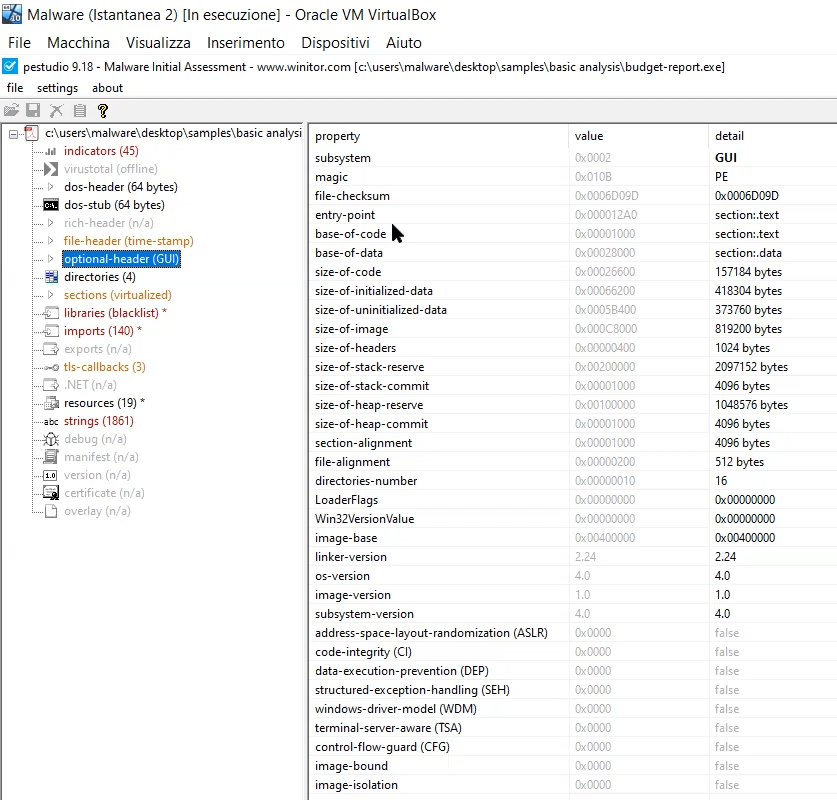
\includegraphics[width=1\textwidth]{images/13-10/3.png}
    \caption{File budget-report, analisi con PE studio - optional-header.}
\end{figure}

In \textbf{optional-header (GUI)} posso vedere che il campo \textit{magic} assume valore PE (0x10B per 32 bit). L\textit{entry-point}, che è l'indirizzo di memoria da dove il loader deve cominciare a caricare il codice eseguibile, combacia (fortunatamente) con l'inizio della sezione .text. L'\textit{image-base} ha valore 0x00400000. 

\begin{figure}[p]
    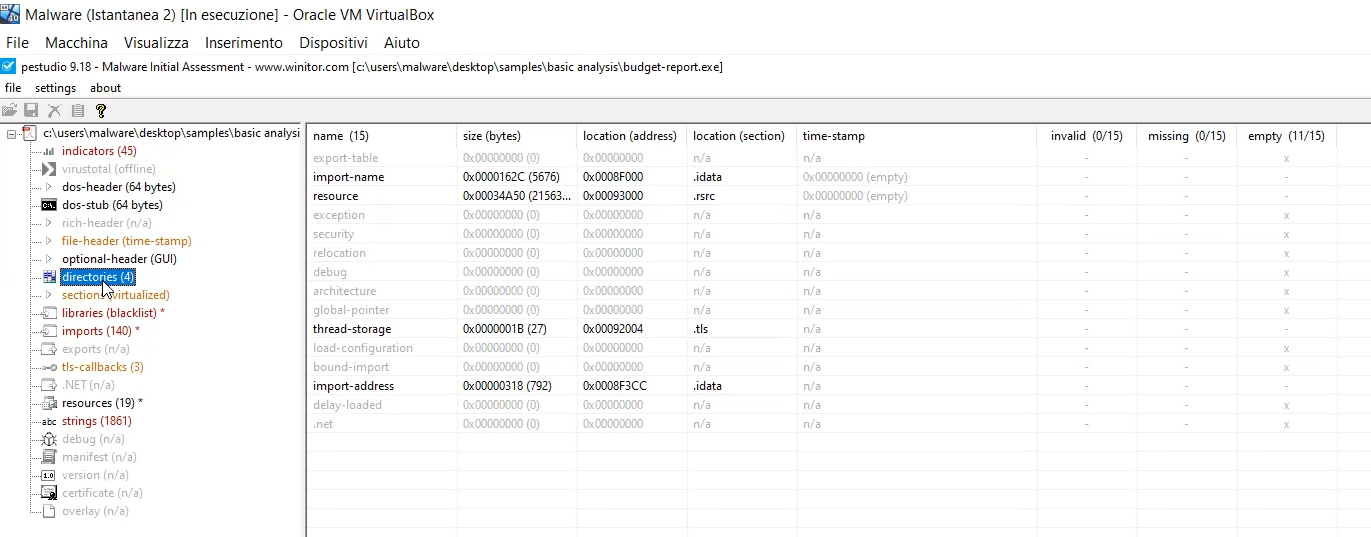
\includegraphics[width=1\textwidth]{images/13-10/4.png}
    \caption{File budget-report, analisi con PE studio - directories.}
\end{figure}

In \textbf{directories}, sono presenti info sulle data directories:
\begin{itemize}
    \item \textit{import-name} è la import table;
    \item \textit{resource} è la resource table;
    \item \textit{import-address} è l'Import Address Table;
\end{itemize}

\begin{figure}[p]
    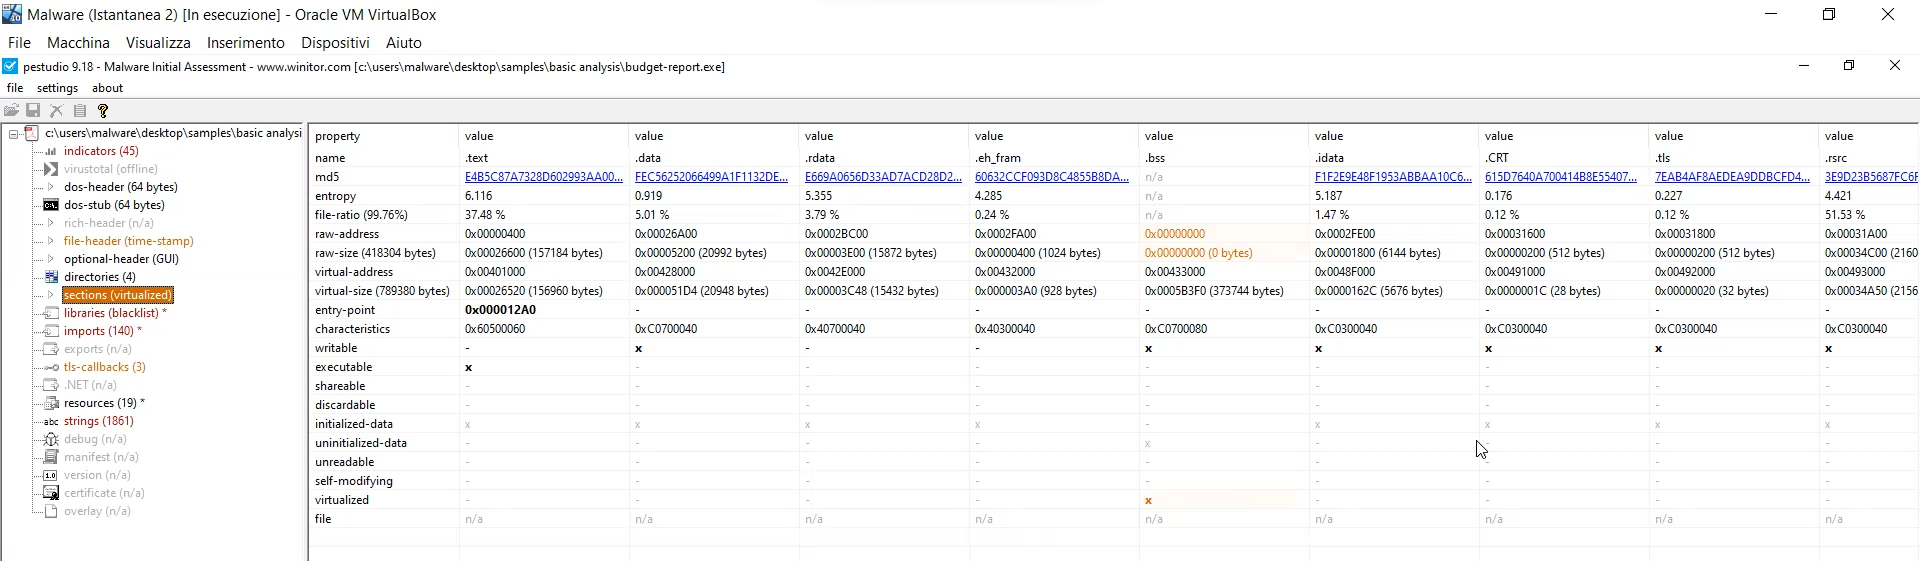
\includegraphics[width=1\textwidth]{images/13-10/5.png}
    \caption{File budget-report, analisi con PE studio - sections.}
\end{figure}

In \textbf{sections (virtualized)} trovo i nomi delle sezioni più delle loro informazioni. Non noto nulla di strano nelle sezioni: .text ha i permessi di esecuzione come dovrebbe e lo stesso vale per .data con quelli di scrittura.

Osservo ora l'Import Address Table. PEStudio la divide in 2 parti: le librerie e le funzioni che queste richiamano. In entrambi i casi, PEStudio andrà a marcare le entry possibilmente malevole.

\begin{figure}[p]
    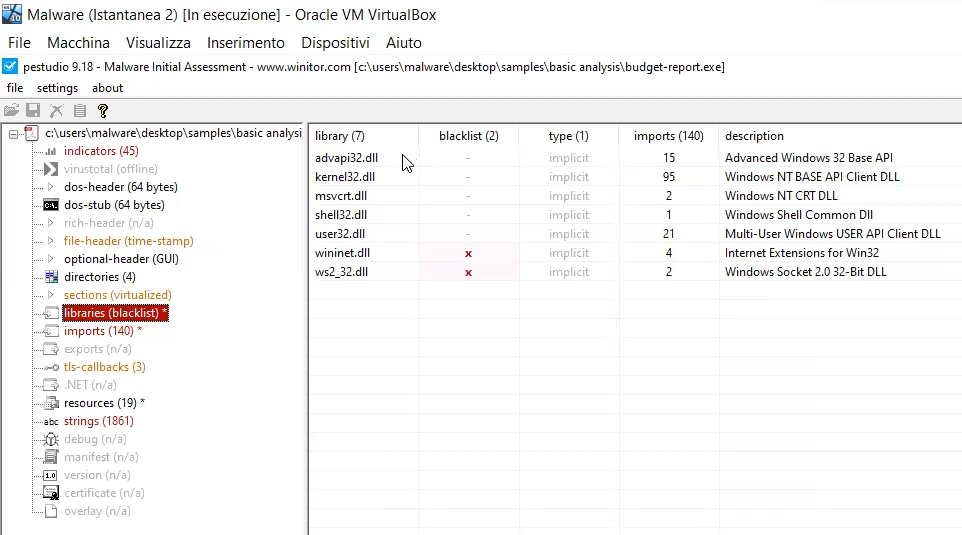
\includegraphics[width=1\textwidth]{images/13-10/6.png}
    \caption{File budget-report, analisi con PE studio - libraries.}
\end{figure}

Le librerie richiamate sono quelle viste nella tabella 1. Noto che tra quelle richiamate sono presenti 2 librerie particolari: \textbf{wininet.dll} e \textbf{ws2\_32.dll}. Entrambe sono collegate alle connessioni di rete, quindi mi posso aspettare che il malware tenterà di creare una connessione di rete

\begin{figure}[p]
    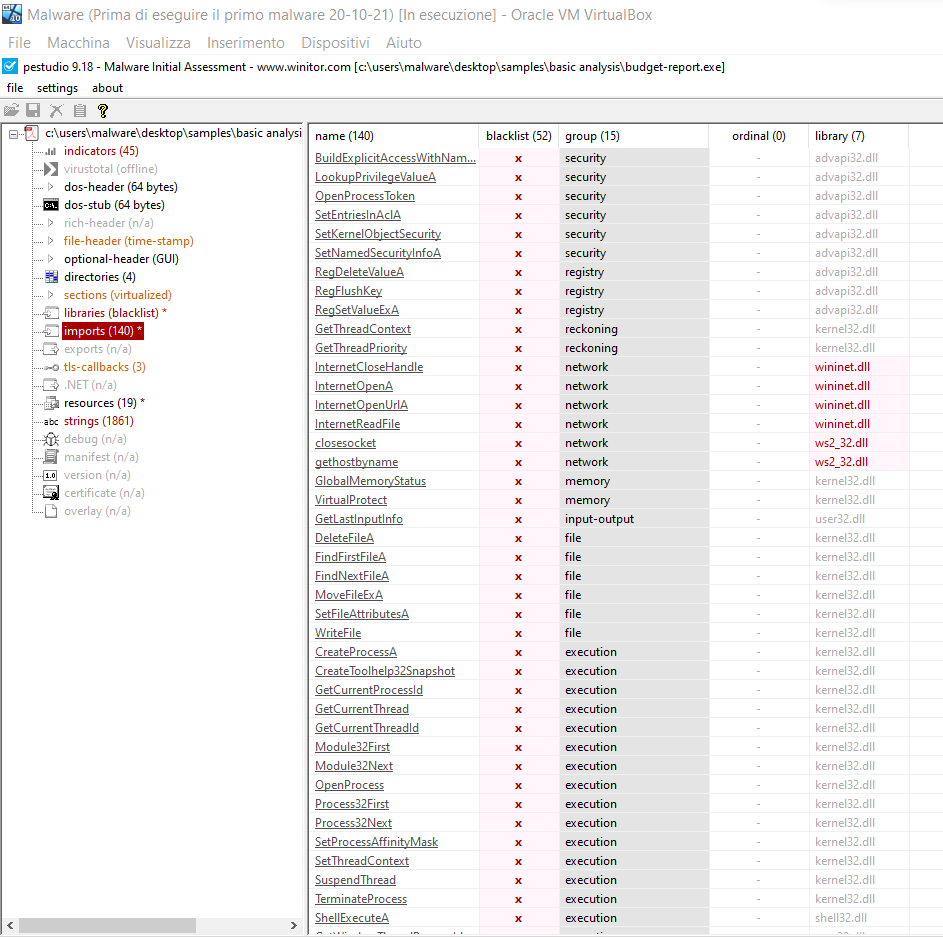
\includegraphics[width=1\textwidth]{images/13-10/7.png}
    \caption{File budget-report, analisi con PE studio - imports.}
\end{figure}

Tra le funzioni richiamate, vado a cercare quelle possibilmente malevole (quelle viste nell'immagine). Tra queste trovo funzioni che operano dei registri di Windows (funzioni che iniziano con reg), funzioni che operano sui file, funzioni che operano con le connessioni, funzioni che operano sulla RAM e funzioni legate alla creazione di processi.

Trovo anche la funzione \textbf{sleep( )}, che è spesso usata nei malware per rimanere dormienti per un po' di tempo ed evitare la detection da parte di programmi anti-malware.

La presenza della funzione \textbf{ShellExecuteA( )} indica che il malware può eseguire programmi. 

Finita questa prima analisi, vado ora a cercare se sono presenti le librerie che permettono di caricare a runtime. Trono la \textit{dynamic-library} e soprattutto le funzioni \textbf{LoadLibraryA} e \textbf{LoadLibraryW}. La differenza tra le due sta nel tipo di stringhe che prendono in input (A per ASCII, W per Unicode). La stringa indica il nome della libreria che deve essere caricata a runtime. 

Dalle librerie scoperta (probabilmente ce ne sono altre possibilmente malevole), posso ipotizzare che il malware: modifichi i registri, crei/acceda ai file, esegua programmi, crei connessioni di rete.

\begin{figure}[p]
    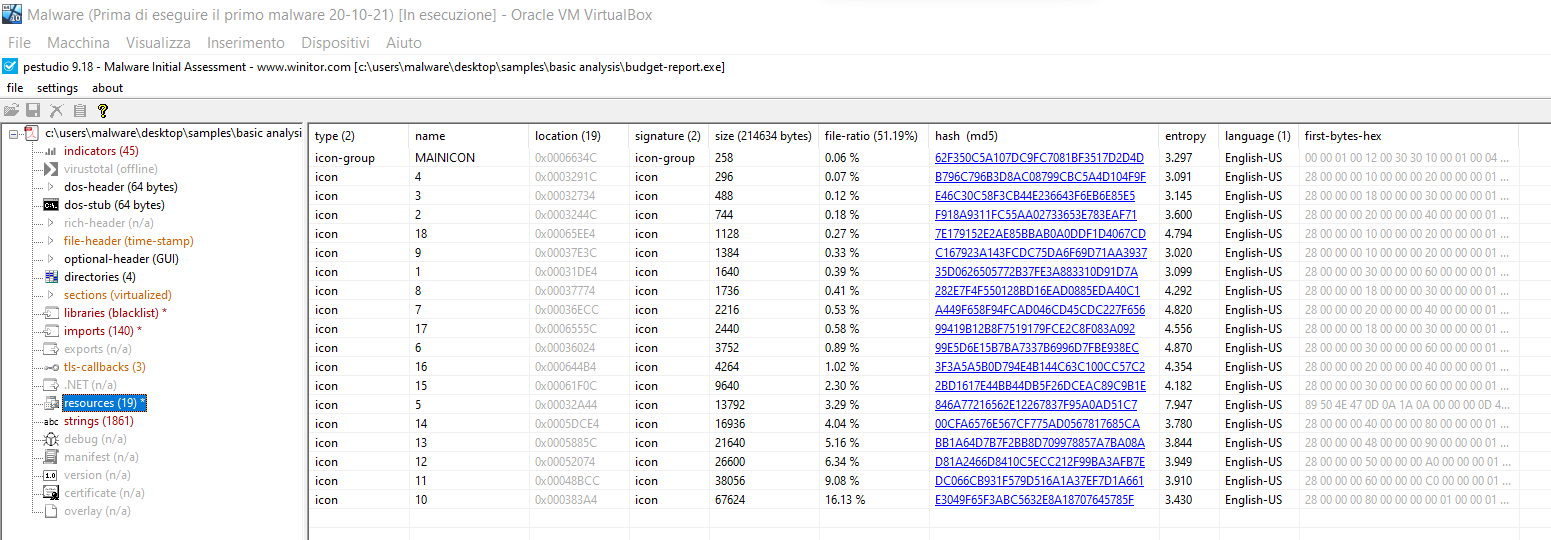
\includegraphics[width=1\textwidth]{images/13-10/8.png}
    \caption{File budget-report, analisi con PE studio - resources.}
\end{figure}

Osserviamo ora le risorse (\textit{resources}). Non noto nulla di strano (il tipo delle risorse è icona, confermato dalla loro signature, e il linguaggio è inglese - non russo o affini). 

Analizziamo ora le stringhe. Tra queste sono presenti:
\begin{itemize}
    \item "connect" e "send", che  potrebbero essere ricollegate a delle funzioni di rete;
    \item "HKLM" e "HKCU", che sono 2 registri di Windows (Local Machine e Current User);
    \item "ABCDEFGHIJKLMNOPQRSTUVWXYZABCDEFGHIJKLMNOPQRSTUVWXYZ0123456789+/", che mi indica che potrebbero esserci delle stringhe codificate in base 64;
    \item "SOFTWARE$\backslash$Microsoft$\backslash$WindowsNT$\backslash$CurrentVersion", che è un registro di Windows;
    \item Una serie di nomi di programmi (opera.exe, ...), che potrebbero indicare che il malware potrebbe controlare lo loro presenza sulla macchina o fare program injection, sostituendosi a essi;
    \item Stringhe HTTP/URL spezzate in più entry;
    \item "autoruns.exe", che è interessante in quanto viene usato spesso per identificare tutte le strategie che il malware ha usato per raggiungere la persistenza sulla macchina. In questo caso il malware potrebbe volerlo stoppare;
    \item Delle directory/percorsi, che potrebbero star ad indicare file che il malware vuole copiare nella macchina infetta;
    \item Funzioni C per l'allocazione dinamica della memoria;
    \item Stringhe legate a nomi di registri di Windows (spezzati in più entry), come "RunO", che sta per Run Ones, o "Policies$\backslash$Explorer$\backslash$RufSoftware$\backslash$Microsoft$\backslash$WindowsNT$\backslash$CurrentVersion";
\end{itemize}

Nel caso siano presenti come stringhe nomi di API non riportate nella Import Table, significa che quelle funzioni vengono caricate a runtime. 

\subsection{Analisi "basic analysis$\backslash$financials-xls"}

\begin{figure}[p]
    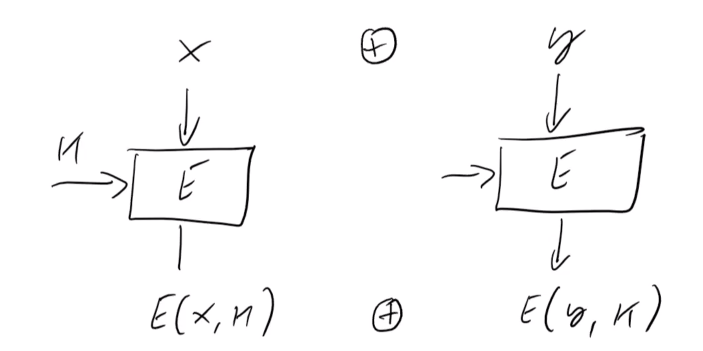
\includegraphics[width=1\textwidth]{images/14-10/1.png}
    \caption{File financials-xls, analisi con PE studio - main.}
\end{figure}

Analizzo con PEstudio. Noto che il malware è impacchettato con UPX (proprietà \textit{signature}). 
Provo a cercare se ci sono altre info nel PE file che mi aiutano a capire se il malware è impacchettato. Questi sono i passi da seguire quando non so con cosa è stato impacchettato il malware. 

\begin{figure}[p]
    \includegraphics[width=1\textwidth]{images/14-10/2.png}
    \caption{File financials-xls, analisi con PE studio - sections.}
\end{figure}

Nelle sezioni (tralasciando il fatto che due si chiamano UPX1 e UPX2). Noto che due di queste possiedono sia il permesso di esecuzione che di scrittura. Solitamente o ho esecuzione+lettura o ho scrittura (campanello di allarme per impacchettatura malware).

\begin{figure}[p]
    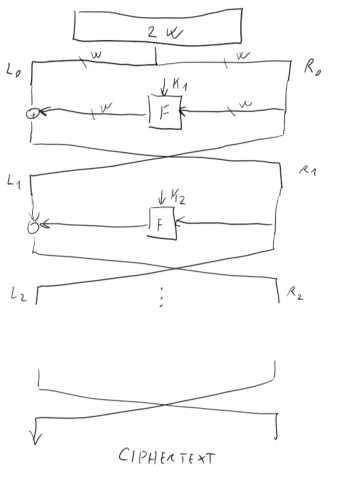
\includegraphics[width=1\textwidth]{images/14-10/3.png}
    \caption{File financials-xls, analisi con PE studio - imports.}
\end{figure}

Osservo ora la Import Address Table. Cedo che ci sono un numero limitato di funzioni che vengono richiamate (campanello di allarme per impacchettatura). Tra le funzioni richiamate troviamo LoadLibraryA e ProcAddress, che sono due delle tre funzioni solitamente richiamate quando il malware è impacchettato.

\begin{figure}[p]
    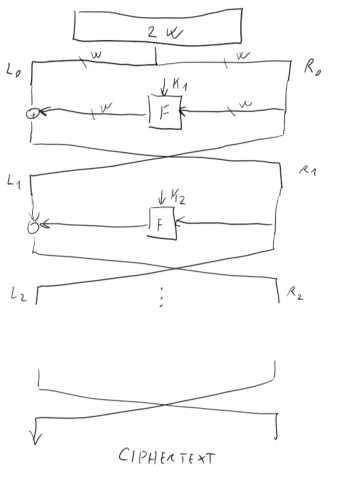
\includegraphics[width=1\textwidth]{images/14-10/3.png}
    \caption{File financials-xls, analisi con PE studio - strings.}
\end{figure}

Tra le stringhe, ne trovo molte di incomprensibili (campanellod i allarme per impacchettatura).

\\
\begin{figure}[p]
    \includegraphics[width=1\textwidth]{images/14-10/4.png}
    \caption{File financials-xls, spacchettamento con UPX.}
\end{figure}

Voglio ora spacchettare il malware. Per farlo uso UPX, che funge sia da impacchettatore che da spacchettatore. Apro la cartella del tool da CMD e eseguo il comando:
\begin{lstlisting}
upx -d -o percorso_dove_spacchettare\nome_spacchettato file_da_spacchettare 
\end{lstlisting}

\begin{figure}[p]
    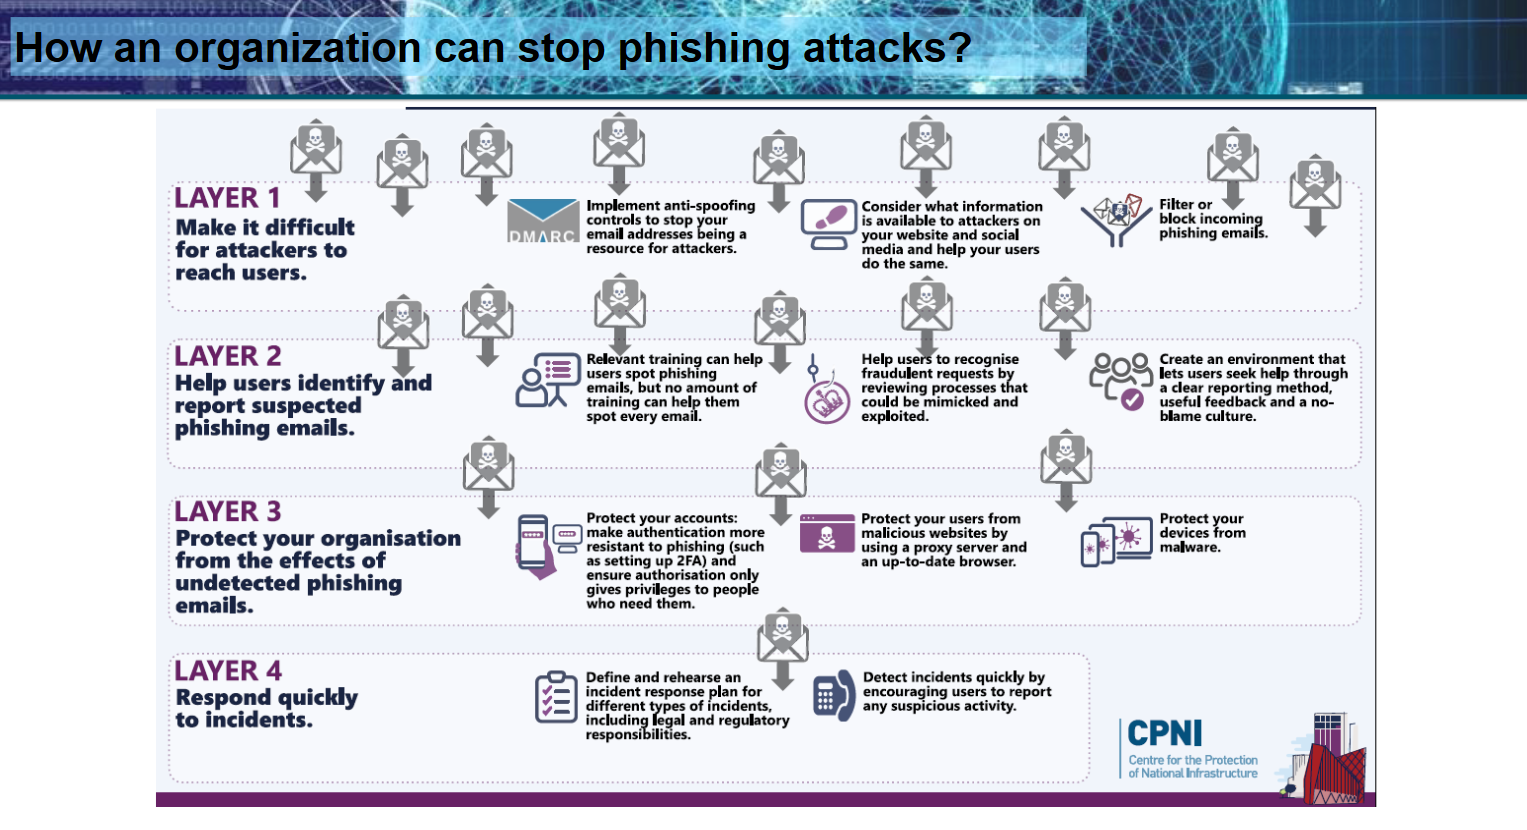
\includegraphics[width=1\textwidth]{images/14-10/5.png}
    \caption{File financials-xls spaccehttato - main.}
\end{figure}

Apro il file spacchettato con PEstudio. Vedo ora che in \textit{signature} non è più presente UPX, che il file è ancora un eseguibile e che ha un'interfaccia grafica (\textit{subsystem}: GUI).











\chapter{Analisi dinamica di base}

Fase in cui sis studia come il malware modifica il file system e/o si connette alla rete. In particolare siamo interessati a verificare se:
\begin{itemize}
    \item Il malware modifica i file sulla macchina o ne crea di nuovi;
    \item Il malware modifica i registri della macchina, per ottenere persistenza;
    \item Il malware genera traffico di rete. Si tratta del modo migliore per capire il suo comportamento;
    \item Il malware lancia altri processi;
    \item Come il malware ottiene persistenza.
\end{itemize}

\section{Windows API}
Le Windows API non usano i classici tipi della programmazione, ma 4 tipi principali:

\begin{table}[h]
    \centering
    \begin{tabular}{c|c}
        WORD (w)     &  intero a 16 bit senza segno\\
        DWORD  (dw)   & intero a 32 bit senza segno\\
        Handle  (H) & puntatore a \underline{oggetti} di Windows (file, interfacce, socket, processi)\\
        Long Pointer (LP) & puntatore ad altri tipi di dato (byte, stringhe)
    \end{tabular}
\end{table}

Gli Handle sono sono puntatori a oggetti che possono essere usati solo per accedere all'oggetto a cui sono associati tramite una funzione di chiamata.

Tra le API pericolose, oltre a quelle legate ai file, ci sono \textbf{CreateFileMapping} e \textbf{MapViewOfFile}, che il malware può usare per emulare lo stesso comportamento dell'operating system loader. La \textbf{CreateFileMapping} è usata per caricare il file interessato nella RAM, mentre la \textbf{MapViewOfFile} è usata per accedere all'area di memoria in cui il file è stato caricato (ritorna l'indirizzo di memoria dove il file è stato caricato). 

\section{Registri di Windows}
Tipicamente contengono impostazioni di configurazione del sistema operativo e dei programmi (es: con quale programma aprire un dato tipo di file) o info su quali programmi avviare allo start del sistema, ad esempio.

I registri sono organizzati gerarchicamente similmente al file system. Le 5 Root Keys (cartelle all'apice) sono:
\begin{itemize}
    \item HKEY\_LOCAL\_MACHINE: contiene le impostazioni globali della macchina; 
    \item HKEY\_CLASSES\_ROOT: contiene le info su quali programmi usare per aprire un dato tipo di file;
    \item HKEY\_CURRENT\_USER: contiene le info sull'utente corrente (es: impostazioni della tastiera)
    \item HKEY\_USERS: contiene le info su tutti gli utente creati. Il current user è una copia di uno degli utenti elencati qui;
    \item HKEY\_CURRENT\_CONFIG: contiene le impostazioni correnti sull'HW della macchina
\end{itemize}

A loro volta le Root Keys contengono una serie di Keys (cartelle), che a loro volta contengono delle Subkeys (sottocartelle). Ad ogni cartella (root key, key, subkey) sono associate una o più entry formate da un Name, un Type e un Data (o Value). 
\\

Generalmente, i malware operano su \textbf{CURRENT\_USER} e \textbf{LOCAL\_MACHINE}, in quanto non richiedono permessi di amministratore

Tra le chiavi più usate c'è \textbf{HKLM$\backslash$SOFTWARE$\backslash$Microsoft$\backslash$Windows$\backslash$CurrentVersion$\backslash$Run} che contiene i programmi da avviare allo start del sistema operativo;
 
\textbf{Autoruns}, un Sysinternal tool di Windows, può aiutare a identificare tutti i possibili modi in cui il malware raggiunge persistenza. Scannerizza i registri, i task e i servizi creati di recente.

Le funzioni legate ai registri più usate sono:
\begin{itemize}
    \item RegOpenKeyEx: apre una chiave esistene per modificarla o interrogarla;
    \item RegSetValueEx: aggiunge una nuova chiave al registro e ne setta il valore Data;
    \item RegGetValue: ritorna il campo Data di un registro esistente.
\end{itemize}

\section{API per le connessioni di rete}
I DLL principali sono

\section{Behavioural Monitoring}
Il controllo del comportamento permette di tracciare tutte le volte in cui i processi in esecuzione sulla macchina usano una certa API. Se un processo chiama, ad esempio, CreateFile( ) per accedere ad un file, è possibile vederlo. Questa tecnica vede anche i file temporanei, ma allo stesso modi della System Integrity Monitoring, viene bypassata dai rootik (copiano file sul kernel non usando le API standard). 
\\

Tramite il tool \textbf{Process Monitor (Procmon)}, fornito di base da Windows, si possono vedere i file creati/cancellati da un processo, tutte le modifiche ai registri, tutti i processi creati e le connessioni di rete iniziate. IL tool permette, tramite filtraggio, di concentrarsi a determinate funzioni di determinate API.

\section{Simulazione di connessione di rete + Esempio completo}
Per simulare le connessioni di rete uso \textbf{fakenet}. Lo runno come amministratore.
\\

Passi:
\begin{enumerate}
    \item Avvio come amministratore fakenet;
    \item Avvio Regshot x86 Unicode come amministratore. Setto come bersaglio l'intero disco C;
    \item Avvio ProcessMonitor come amministratore e lo stoppo;
    \item Fatto il primo shot con Regshot;
    \item Faccio partire la cattura con Procmon;
    \item Lancio il malware e attendo 5 minuti affinchè esegua;
    \item Stoppo la cattura di Procmon;
    \item Faccio il secondo shot e comparo i 2.
\end{enumerate}

\chapter{Esercitazione Analisi dinamica di base}

\section{System Integrity Monitoring}
Eseguo \textbf{Regshot 1.9.0 x86 Unicode} come amministratore. Checko \textit{scan dir1[dir2;...]} e modifico il percorso in "C:$\backslash$". Premo \textit{first shot}.
\begin{center}
    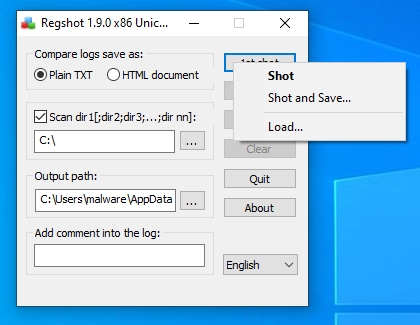
\includegraphics[]{images/20-10/1.png}
\end{center}

Eseguo ora il malware. Il malware sparisce. Aspetto 5 minuti per lasciare che esegua tutte (si spera) le sue istruzioni. Faccio una seconda istantanea con \textbf{Regshot}.
\\

Comparo le due snapshot usando \textit{compare}. 

\begin{center}
    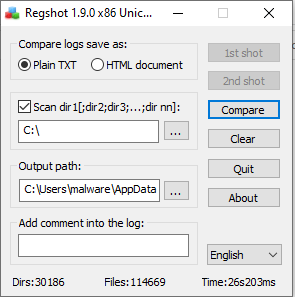
\includegraphics[]{images/20-10/2.png}
\end{center}
Nel file di testo che contiene la comparazione, nella sezione "Folders added", posso notare che vi è una entry che differisce dalle altre della sezione (nel video della lezione c'erano più entry non legate al malware), ovvero la cartella "C:$\backslash$Users$\backslash$malware$\backslash$AppData$\backslash$Roaming$\backslash$12648430".\\
\begin{center}
    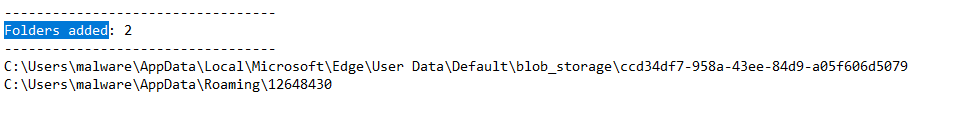
\includegraphics[width=1\textwidth]{images/20-10/3.png}
\end{center}
Se vado ora nella sezione "Files added", vedo che la cartella creata prima è presente anche qui e contiene un file, "spoolsv.exe".
\begin{center}
    \includegraphics[width=1\textwidth]{images/20-10/4.png}
\end{center}
Se vado in "Files deleted", ho la conferma che il malware è stato cancellato.

In "Values added" (relativi ai registri), vedo che la cartalla creata "12648430" è presente in più entry. 
Vedo che è stata creata una chiave che contiene il nome della cartella con valore una stringa, che a occhio sembra codificata. Inoltre al registro \textbf{RunOnce} è stata aggiunta una nuova chiave che ha come percorso il file "spoolsv".

\begin{center}
    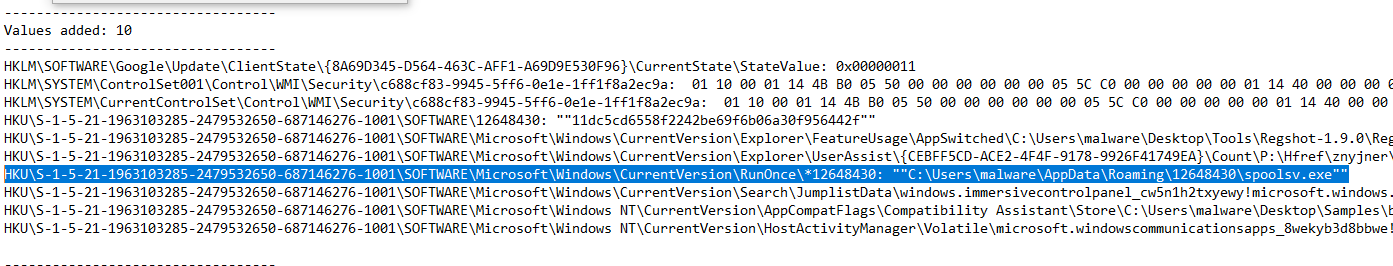
\includegraphics[width=1\textwidth]{images/20-10/5.png}
\end{center}
Posso quindi ipotizzare che il malware, una volta eseguito, cancelli se stesso, crei una nuova cartella in "Roaming" e vi piazzi all'interno un eseguibile, ed raggiunge persistenza sulla macchina creando una nuova chiave di registro in \textbf{RunOnce} di \textbf{HKU}.
\\

Se vado ora in "C:$\backslash$Users$\backslash$malware$\backslash$AppData$\backslash$Roaming" non vedo la cartella "12648430". Teoricamente dovrei vederla tra le cartelle nascoste. Calcolando l'hash dell'eseguibile al suo interno e confrontandolo col malware originale, dovrei vedere che è lo stesso (i due programmi sono uguali).

\section{Behavioural Monitoring}

Eseguo \textbf{Procmon} come amministratore. Di base il tool cattura migliaia di eventi al secondo. Premendo su simbolo con la forma di \textit{diamante}, è possibile accedere alla schermata dei filtri. 

Provo ad aggiungere vari filtri:
\begin{enumerate}
    \item Filtro per ProcessName il processo winlogon.exe;
    \item Filtro per la funzione WriteFile. Le funzioni stanno sotto l'opzione Operation;
    \item Filtro per la funzione RegSetValue;
    \item Filtro per la funzione Process Create;
    \item Filtro per la funzione SetDispositionInformationFile, per tracciare la cancellazione di file;
    \item Filtro per tutte le operazioni che cominciano con TCP.
\end{enumerate}
\\

Avvio Procmon con  i filtri di prima, tranne per ProcessName, che cambio con "budget-report.exe". Eseguo "budget-report". Lo faccio andare per qualche minuto. Stoppo Procmon. 

In ordine di tempo (dalla più vecchia alla più nuova) vedo che il malware:
\begin{enumerate}
    \item Scrive su un file di log "C:$\backslash$Users$\backslash$malware$\backslash$ntuser.dat.LOG2" con WriteFile( );
    \item Setta il valore nella chiave di registro "HKCU$\backslash$SOFTWARE$\backslash$12648430";
    \item Riscrive sul file di log;
    \item Setta il valore della chiave "HKCU$\backslash$SOFTWARE$\backslash$Miscrosoft$\backslash$CurrentVersion$\backslash$Explorer$\backslash$Advanced$\backslash$Hidden". Questa chiave di registro riguarda la tipologia di visualizzazione dei file nascosti. Visualizzando la entry posso vedere il valore che le è stato assegnato, che in questo caso rende i file \textit{hidden};
    \item Crea un file temporaneo "C:$\backslash$Users$\backslash$malware$\backslash$AppData$\backslash$Local$\backslash$Temp$\backslash$12648030.bat";
    \item Modifica i valori di alcuni registri legati alle connessioni di rete;
    \item Apre il cmd con parametro il file .bat che ha creato;
    \item Raggiunge persistenza andando a creare una chiave nel registro RunOnce. Come valore della chiave ha inserito il percorso alla copia di se stesso che ha creato nella cartella Roaming di AppData;
\end{enumerate}

\section{Esempio completo con connessione di rete simulata}
Passi:
\begin{enumerate}
    \item Avvio come amministratore fakenet;
    \item Avvio Regshot x86 Unicode come amministratore. Setto come bersaglio l'intero disco C;
    \item Avvio ProcessMonitor come amministratore e lo stoppo;
    \item Fatto il primo shot con Regshot;
    \item Faccio partire la cattura con Procmon;
    \item Lancio \textbf{financials-xls} e attendo 5 minuti affinchè esegua;
    \item Stoppo la cattura di Procmon;
    \item Faccio il secondo shot e comparo i 2.
\end{enumerate}

Guardando i risultate del compare di Regshot, vedo che è stata aggiunta una nuova chiave di registro sotto quello che potrebbe essere l'utente corrente, con valore "C:$\backslash$Windows$\backslash$xpupdate.exe". Questo potrebbe essere il modo con cui il malware raggiunge persistenza. Se guando però sotto la sezione "Files added", non lo trovo. 

Da Procmon, oltre la conferma della creazione della chiave, vedo che il malware ha eseguito alcune operazioni TCP. Neanche qua ho info sulla creazione di "xpupdate.exe".
\\

Provo ora ad eseguire il malware con privilegi di amministratore. Ora, sia Regshot che Procmon confermano al creazione del file "C:$\backslash$Windows$\backslash$xpupdate.exe". Probabilmente per raggiungere la persistenza il malware aveva bisogno di essere eseguito con i permessi di amministratore.
Con l'esecuzione normale infatti poteva solo creare la chiave di registro per la persistenza, ma non il file effettivo da far persistere. 
\\

In entrambe le esecuzioni, crea un file "C:$\backslash$Users$\backslash$malware$\backslash$AppData$\backslash$Roaming$\backslash$Install.dat" e mantiene la persistenza del file originale aggiungendo una chiave di registro in HKU.
\\

Confrontando "xpupdate.exe" e "financials-xls" con ComputeHash, ottengo lo stesso hash. Quindi i 2 file sono uguali.

\section{File esame 2019 - sample1}

\begin{enumerate}
    \item Avvio come amministratore fakenet;
    \item Avvio Regshot x86 Unicode come amministratore. Setto come bersaglio l'intero disco C;
    \item Avvio ProcessMonitor come amministratore e lo stoppo;
    \item Fatto il primo shot con Regshot;
    \item Faccio partire la cattura con Procmon;
    \item Lancio \textbf{sample1} come AMMINISTRATORE e attendo 5 minuti affinchè esegua;
    \item Stoppo la cattura di Procmon;
    \item Faccio il secondo shot e comparo i 2.
\end{enumerate}

Dal Regshot vedo che il malware crea un file "C:$\backslash$Windows$\backslash$lsass.exe".

\end{document}